%\documentclass[preprint]{iucr}              % DO NOT DELETE THIS LINE
\documentclass{iucr}              % DO NOT DELETE THIS LINE

\usepackage{siunitx}
\usepackage{color}
% \usepackage{amsmath,amssymb}
\usepackage{mathtools}
\usepackage[normalem]{ulem}

% rotation table labels...
% see https://tex.stackexchange.com/questions/98388/how-to-make-table-with-rotated-table-headers-in-latex
\usepackage{adjustbox}
\usepackage{array}
\usepackage{booktabs}
\usepackage{multirow}

%
%

\newcommand{\todo}[1]{{\color{red}[TODO: "#1'']}}
\newcommand{\inblue}[1]{{\color{blue}#1}}
\newcommand{\inred}[1]{{\color{red}#1}}
\newcommand{\ingreen}[1]{{\color{green}#1}}
\newcommand{\soutred}[1]{{\color{red}\sout{#1}}}

\definecolor{JSR_blue}{RGB}{51, 102, 154}
\newcommand{\jsrblue}[1]{\textcolor{JSR_blue}{#1}}

\newcolumntype{R}[2]{%
    >{\adjustbox{angle=#1,lap=\width-(#2)}\bgroup}%
    l%
    <{\egroup}%
}
\newcommand*\rot{\multicolumn{1}{R{90}{1em}}
%
}
\journalcode{S}


\begin{document}                  % DO NOT DELETE THIS LINE

\title{Focusing partially-coherent x-ray beams with lenses. Multi-optics simulations.}

\cauthor[]{\jsrblue{Manuel}}{\jsrblue{Sanchez del Rio}}{srio@esrf.eu}{address if different from \aff}
\author[]{\jsrblue{Rafael}}{\jsrblue{Celestre}}
\author[]{\jsrblue{Juan}}{\jsrblue{Reyes-Herrera}}
\author[]{\newline \jsrblue{Philipp}}{\jsrblue{Brumund}}
\author[]{\jsrblue{Marco}}{\jsrblue{Cammarata}}

\aff[]{ESRF - The European Synchrotron, 71 Avenue des Martyrs, 38000 Grenoble, \country{France}}

\maketitle                        % DO NOT DELETE THIS LINE

% -----------------------------------------------------------------
% -----------------------------------------------------------------

\begin{synopsis}
Simulations of focusing partial coherent beams with x-ray lenses are performed with different software packages (ShadowOui, SRW, COMSYYL and WOFRY). The four codes give comparable results, that are discussed in detail. 
\end{synopsis}

% -----------------------------------------------------------------
% -----------------------------------------------------------------

\begin{abstract}
We simulate the focusing of the radiation produced by fourth-generation storage rings with multiple optics packages implementing a variety of methods for dealing with partial coherence. Ray-tracing uses a hybrid algorithm combining geometrical optics with wave optics corrections. Other codes propagate a set of wavefronts describing the undulator emission. A Monte-Carlo method combine wavefronts from electrons entering to the undulator with different values. Two packages perform coherent mode decomposition of the undulator radiation in 1D and 2D dimensions. The four codes give comparable results for four different setups of an optical system composed by a slit and two beryllium lenses.
\end{abstract}

% -----------------------------------------------------------------
% -----------------------------------------------------------------

\section{Introduction}
\label{sec:introduction}

Diffraction effects produced when propagating x-ray beams along beamline components are fundamental for the 
recent fourth-generation storage-ring-based X-ray synchrotron sources. The transversal coherence of these beams is highly improved, in particular in the horizontal direction, with respect to previous 3$^{\text{rd}}$ generation sources.
Preserving wavefront quality requires better quality materials and optical surfaces in the active beamline components such as mirrors, gratings, crystals and lenses \cite{Yabashi, Roth2017}.

The effect of radiation coherence is evident in the new synchrotron sources. For example, in case of a focusing system made by a mirror or lens that focuses the source into the image plane. If the numerical aperture (NA) is reduced (for example by the finite dimension of the lens, mirror or by using a slit upstream from the lens) the position and dimensions of the focused beam are altered due to diffraction. This is relevant for synchrotron beamlines, as demonstrated by \citeasnoun{westfahl}, who noticed a shift of the horizontal focal position upstream from the position given by geometrical optics (see Fig. 7 in \citeasnoun{westfahl}) when the horizontal acceptance is reduced by a slit. Their numeric results from wavefront propagation using SRW \cite{codeSRW} including partial coherence agree with an analytical Gaussian Shell-model.

The diffraction effects in synchrotron radiation cannot be simulated by the limiting cases of full incoherence (usually simulated by geometrical ray-tracing) or by propagating a single wavefront, valid for fully coherent radiation. The coherent fraction of the radiation emitted by new generation storage rings, although much improved with respect to previous generations, is still of the order of a few per cent at hard x-rays. This imply that none of geometrical optics of coherent wavefront propagation describe correctly the beam transport along a typical beamline. Partial coherence should be taken into account, complicating the simulation processes. In the last years several approaches have demonstrated to work for beamlines using undulator radiation. Starting from incoherent beams, \citeasnoun{codeHYBRID} proposed some correction algorithms to include diffraction effects that happen with coherent radiation. More accurate methodologies start from coherent wavefront propagation. The partial coherence is included by propagating a set of wavefronts that all together describe the undulator radiation. Two approaches are possible: calculating the wavefronts emitted by electrons entering in the undulator with different initial conditions, sampled by Monte Carlo from the electron beam emittance (multi-electron in SRW) \cite{codeSRW_ME}, and assigning these wavefronts to the coherent modes, eigenfunctions numerically obtained from making a coherent mode decomposition of the undulator source \cite{codeCOMSYL}.  

In this paper we study the propagation of a partial coherent beam in the context of the project for the new ID18 beamline at the upgraded EBS-ESRF storage ring. We have compared results for different setups composed by two refractive systems (transfocators), plus a slit placed upstream from the transfocators. The focal spots produced by four different transfocator configuratiuons are studied in detail using four packages: i) hybrid ray-tracing as described by \citeasnoun{codeHYBRID} and implemented in ShadowOUI \cite{codeSHADOWOUI}; ii) multi-electron simulations as implemented in SRW \cite{codeSRW}; iii) full coherent mode decomposition (in 2D) made by the code COMSYL \cite{codeCOMSYL} and then propagated using WOFRY \cite{codeWOFRY}; and iv) a novel 1D coherent mode decomposition also implemented in WOFRY, and based on the previous method but allowing interactive simulations. 

% To study the performances of such systems a new algorithm for coherent mode decomposition (CMD) of the undulator beams has been developed. This method is very fast allowing parametric simulations in a common laptop.

% The high efficiency of the CMD software developed is obtained by implementing a 1D model, therefore studying separately the horizontal and vertical planes. 

% Simulation of the source include coherent mode decomposition (CMD) using COMSYL \cite{codeCOMSYL}, or Monte-Carlo multi-electron propagation with SRW \cite{codeSRW}. It is also found that ray-tracing simulations using the ``hybrid" method \cite{codeHYBRID} give good approximations to the correct results for these systems. A simplified algorithm for CMD in 1D is available in WOFRY. It is very fast allowing parametric simulations in a common laptop, with results in good agreement with the other methods that require a computing cluster.

% The paper is organized as follows. Section~\ref{sec:theory} summarizes the methodology used for 1D coherent mode decomposition of undulator beams and their transport along the beamline. Section~\ref{sec:onelens} analyzes the focusing of partially-coherent beams with a single refractive system (lens). Section~\ref{sec:twolenses} discusses the pairing of two refractive systems. Section~\ref{sec:complete-beamline} shows simulations for the full beamline and compares different methodologies for a selected case. We finish with a general discussion in Section~\ref{sec:discussion} and  concluding remarks in Section~\ref{sec:summary}. 

% -----------------------------------------------------------------
% -----------------------------------------------------------------

\section{Methods to describe partial coherent beams from undulators in a storege ring}
 \newline
We introduce four different methods used for dealing with partially-coherent beams emitted by undulators in low-emittance storage rings: hybrid ray-tracing in ShadowOUI; Monte Carlo multi-electron simulations as implemented in SRW; a 2D-CDM method implemented in COMSYL; and the proposed 1D-CMD method separating the horizontal- and vertical-directions implemented in WOFRY. 

These four methods have their independent distribution managed by their authors, but are conveniently grouped together within the OASYS suit \cite{codeOASYS}.



% We introduce the different methods used for dealing with partially-coherent beams emitted by undulators in low-emittance storage rings: hybrid ray-tracing in ShadowOUI, Monte Carlo multi-electron simulations as implemented in SRW, and CMD, as implemented in COMSYL (2D) and WOFRY (1D). 


\subsection{Hybrid ray-tracing (ShadowOUI)}

The use of pure ray-tracing methods (based in geometrical optics) is not adequate when analyzing optical systems dealing with coherent beams (originating diffraction effects). Conventional ray-tracing does not reproduce the effects of focal position shift and focus degradation when the NA is reduced. However, ray-tracing-based methods are much simpler and fast than wave-optics-based methods and in many occasions they are very useful to evaluate the impact of the beam coherence when studying a synchrotron beamline. Because of that, a hybrid \cite{codeHYBRID} algorithm has been developed, incorporating concepts of coherent diffraction in the ray-tracing code SHADOW \cite{codeSHADOW}. It is fully integrated in the ShadowOUI \cite{codeSHADOWOUI} add-on in OASYS. It has been demonstrated to be an efficient and fast tool to design beamlines also including coherence effects. The hybrid ray-tracing can reproduce the effect of degradation of the focus shift and focal shift when changing the NA. 


\subsection{Multi-electron Monte Carlo (SRW-ME)}



% SRW~\cite{codeSRW} is a well-established code in the synchrotron community for simulating the emission of synchrotron sources and propagating it along a full beamline. It can be used in single-electron (also called filament beam mode or simply SRW-SE) mode, where the source is the fully coherent undulator radiation in an ideal storage ring with zero emittance. To include finite-emittance, and therefore the production and propagation of partial coherent beams, SRW uses the multi-electron (macro-electrons algorithm or SRW-ME) algorithm, that propagates many wavefronts each one created by an electron that enters in the ID with different initial conditions (position and direction) that are sampled from the parameters of the electron beam (moments or Twiss parameters) using a Monte Carlo method \cite{codeSRW_ME}. This method allows to produce accurate intensity maps (by adding the intensity of individual electrons) and is possible to calculate other parameters of the partially-coherent-beam, such as coherence lengths. The SRW-ME requires the use of HPC. 
% However, it is not able to store the 4D CSD nor to calculate the CF. 

In the frequency domain, the synchrotron radiation (SR) intensity from $N_\text{e}$ electrons is given by: 
\begin{equation}
\begin{split}
|E&_{\omega\text{~bunch}}(\textbf{r})|^2 \approx \\
 &N_\text{e} \int\big| E_\omega(\textbf{r};\textbf{s}_\text{e}, \textbf{s}'_\text{e}, \gamma_\text{e})\big|^2\cdot f(\textbf{s}_\text{e}, \textbf{s}'_\text{e}, \gamma_\text{e})~ \text{d}\textbf{s}_\text{e} \text{d}\textbf{s}'_\text{e} \text{d}\gamma_\text{e}~+\\
&+~ N_\text{e}(N_\text{e}-1)\bigg| \int E_\omega(\textbf{r};\textbf{s}_\text{e}, \textbf{s}'_\text{e}, \gamma_\text{e})\cdot f(\textbf{s}_\text{e}, \textbf{s}'_\text{e}, \gamma_\text{e})~ \text{d}\textbf{s}_\text{e} \text{d}\textbf{s}'_\text{e} \text{d}\gamma_\text{e} \bigg|^2,
\end{split}
\label{eq:SR}
\end{equation}
where $E_{\omega\text{~bunch}}(\textbf{r})\equiv E_{\text{~bunch}}(x,y;\omega)$ and $E_\omega(\textbf{r})\equiv E(x,y;\omega)$; $\textbf{s}_\text{e}=(x_\text{e},y_\text{e},z_\text{e})$ represents the electron initial positions, $\textbf{s}'_\text{e}=(x'_\text{e},y'_\text{e})$ gives the electron initial directions and $\gamma_\text{e}$ is the electron energy. All sampled from the 6D electron-beam phase-space such that $\int f(\textbf{s}_\text{e}, \textbf{s}'_\text{e}, \gamma_\text{e})~ \text{d}\textbf{s}_\text{e} \text{d}\textbf{s}'_\text{e} \text{d}\gamma_\text{e}=1$ \cite{codeSRW_CSR}. The methods for computing the spontaneous emission by a relativistic electron submitted to an arbitrary magnetic field, that is $E_\omega(\textbf{r};\textbf{s}_\text{e}, \textbf{s}'_\text{e}, \gamma_\text{e})$, are described in \cite{Chubar1995,codeSRW}.
The first term in the sum from Eq.~\ref{eq:SR} describes temporally incoherent SR, while the second term, temporally coherent SR: $\text{I}_\text{~bunch} = \text{I}_\text{~iSR}+\text{I}_\text{~cSR}$. For emitted wavelengths shorter than the electron bunch length, the power associated with the term $\text{I}_\text{~cSR}$ vanishes quickly \cite{Wiedemann2015}. At typical X-ray energy ranges in the ESRF-EBS, i.e. from a few hundred electron-volts to a few hundred keV, and typical bunch lengths (over 30~ps), $\text{I}_\text{~cSR}$ can be completely neglected even when considering standard monochromatisation schemes in beamlines. A further simplification to Eq.~\ref{eq:SR} is done when considering that the intensity of the single-electron emission is not dependent on the initial electron position $z_\text{e}$. The integration of Eq.~\ref{eq:SR} can then be done in 5 dimensions.

The SRW-ME algorithm used to account for partial (transverse) coherence implements Eq.~\ref{eq:SR} by individually calculating the SR emission of several electrons subjected to the initial conditions sampled from $f(\textbf{s}_\text{e}, \textbf{s}'_\text{e}, \gamma_\text{e})$ passing through an arbitrary magnetic field describing the X-ray source. Each resulting electric field is then propagated through the beamline until the observation point, where the contributions from different electrons are added in intensity \cite{codeSRW_ME}. It is impractical (and unnecessary) to account for the emission of every single electron in a beam that very often has a current of few hundreds mA. Electrons are then divided in so-called macro-electrons (\textit{me's}), which is an abstraction that allows to group the emission of several individual electrons into one particle behaving (in electro-dynamics theory terms) as a single electron emission, but with resulting intensity given by the total intensity $\text{I}_\text{~bunch}$ divided by the number of macro-electrons. An advantage of the SRW-ME approach is that the electric fields of the \textit{me's} propagate independently from each other, which allows a convenient parallelisation of the wavefront propagations among many processors.



% we developed a 1D model of the CMD method that we previously developed in 2D \cite{glass2017}. The motivation for developing these new tools is to perform quick calculations (e.g., being able to perform parametric calculations in a laptop) with high accuracy in the simulation of the source and beam propagation. The separation of the real 2D wavefront in two separated 1D wavefronts is well justified for most synchrotron beamlines, where the cross-talk between these two directions is small. 
% The tools developed here are included in the OASYS toolbox \cite{codeOASYS}, available as an WOFRY add-on. These tools can be used from the OASYS interface, which also creates scripts that can be later modified for performing parametric calculations and loops in batch runs. 


\subsection{Coherent mode decomposition of undulator radiation (COMSYL)}

The electrons in a storage ring are statistically distributed, following in good approximation a Gaussian distribution in a 6-dimensional space (three spatial coordinates, two angles to define direction, and the electron energy). The radiation of the individual electrons will add incoherently for wavelengths smaller than the bunch lengths. This is the usual case for X-rays produced by storage ring-based sources, but not for free electron lasers. Therefore, each electron creates a wavefront (fully coherent) associated at a given photon energy. As a consequence, the overall radiation cannot be described deterministically. Statistical methods are then needed, like for describing the electron beam. This is the origin of partial coherence of the synchrotron emission. In an ideal storage ring of zero emittance, the electrons follow a filament beam so the emission by an insertion device (ID) would be fully coherent. When electron emittance is considered, the electrons contributing to the radiation have different initial conditions (in the 6-dimensional space) and the overall emission cannot be describe by a single wavefront, but by statistically distributed wavefronts, described by partial coherent optics.

The radiation is ``wide sense stationary" \cite{mandel_wolf} if it verifies some conditions, usually satisfied for light emitted by storage rings, but not for XFELs \cite{geloni2008}. These conditions can be summarized as
i) the electron bunch length being long enough (several times larger than the emitted wavelength),
ii) radiation is monochromatized 'not too much' (like by standard monochromators), and 
iii) the radiation frequency being large enough.
It is in this case all the coherent properties of the radiation can be described using $W$, the ``cross spectral density" (CSD), a complex function that measures the correlation of the electric field $E$ in two different spatial points at a given radiation frequency $\omega$. It can be mapped in a $(x,y)$ plane at a third coordinate $z$. At that plane, the CSD depends on 5 variables: 

\begin{equation}
W_{2D}(x_1,y_1,x_2,y_2;\omega) = <E^*(x_1,y_1;\omega) E(x_2,y_2;\omega)>
\label{eq:CSD_1D}
\end{equation}

From the cross spectral density one can calculate the 'spectral density' (usually simply called 'intensity') $I(x,y,\omega)=W_{2D}(x,y,x,y,\omega)$, and also the complex degree of (transverse) coherence: 

\begin{equation}
\mu_{2D}(x_1,y_1,x_2,y_2,\omega) = \frac{W_{2D}(x_1,y_1,x_2,y_2,\omega)}{\sqrt{I_{2D}(x_1,y_1,\omega)}\sqrt{I_{2D}(x_2,y_2,\omega)}}
\label{DTC}
\end{equation}
The modulus of the complex degree of coherence is one for a completely coherent beam and zero for an incoherent beam. 

An important result in partial coherence optics permits to describe the radiation as an infinite sum of independent coherent modes (in the sense of orthonormality) :
\begin{equation}
W_{2D}(x_1,y_1,x_2,y_2,\omega) = \sum_{n=0}^{\infty} \Lambda_n(\omega) \Phi_{n}^*(x_1,y_1,\omega) \Phi_{n}(x_2,y_2,\omega) 
\label{CMD}
\end{equation}
where $\Lambda_n$ (eigenvalues) are the intensity weights and the $\Phi$ are the coherent modes (eigenfunctions). 
Some important characteristics of this coherent mode decomposition are: i) the modes are orthonormal (in the integral sense), ii) the modes maximize the spectral density, the first mode is more intense than the second, and so on, meaning that the truncated expansion is optimal, and iii) there is complete coherence if and only if there is only a single mode. If one can truncate the infinite series to a limited number of modes $N$ which contain a good percentage of the spectral density, the numerical storage of the $N$ modes that depend on two spatial variables is usually more economic than the storage of the cross spectral density $W$ that depends on four variables. 
The eigenvalues $\Lambda_n$ are a measure of the intensity. One can define the occupation $\eta$ of the i-th mode as the normalized intensity: 

\begin{equation}
\eta_i(\omega) = \frac{\Lambda_i(\omega)}{\sum_{n=0}^{\infty} \Lambda_n(\omega)}
\end{equation}

From these arguments, it is now natural to rigorously define Coherent Fraction ($CF_{2D}$) as the occupation of the first coherent mode: $CF_{2D}=\eta_0$.

%%%%%%%%%%%%%%%%%%%%%%%%%%%%%
The interest of the coherent mode decomposition method is twofold: the possibility to propagate a partial coherent beam along the beamline by just propagating a few modes (less modes for a more coherent beam) which behave like coherent wavefronts, and the use of the coherent fraction (a scalar parameter) as a well-defined measure of how coherent is the beam at any position of the beamline.

\subsection{1D coherent mode decomposition: separate horizontal and vertical directions (WOFRY)}

In the following, we suppose that the CSD is separable in its 1D horizontal $x$ and vertical $y$ coordinates, therefore the $W_{2D}$ becomes a product of two CSD functions $W$ of two variables for a given photon frequency $\omega$:

\begin{equation}
W_{2D}(x_1,y_1,x_2,y_2;\omega) = W(x_1,x_2;\omega) W(y_1,y_2;\omega).
\label{eq:CSD_2D}
\end{equation}
Each $W$ function is treated separately in a similar way affecting the $x$ (horizontal) and $y$ (vertical) coordinate. This separation is believed to work well for non-round beams, and for photon energies not far from the undulator resonance \cite{tanaka2014,nash2021}. The CMD for each direction is:
\begin{equation}
W(x_1,x_2;\omega) = \sum_{n=0}^{\infty} \lambda_n(\omega) \phi_n^*(x_1;\omega) \phi_n(x_2;\omega) 
\label{eq:CMD1D}
\end{equation}
with $\lambda_n$ the 1D eigenvalues and $\phi_n$ the 1D eigenfunctions. This gives raise to two values of coherence fraction, for the horizontal and vertical directions, and the 2D CF is the product $CF_{2D}=CF_H \times CF_V$. The $\phi_n$ eigenvectors can be are propagated to any position of the beamline like standard wavefronts. Calling $\phi'$ the wavefront originated by propagating the (source) mode $\phi$, we can construct the propagated CSD    
\begin{equation}
W'(x_1,x_2;\omega) = \sum_{n=0}^{\infty} \lambda_n(\omega) \phi'^{*}_n(x_1;\omega) \phi'_n(x_2;\omega).
\label{eq:propagatedCSD}
\end{equation}
Note that the propagated wavefronts $\phi'$ are in general not orthonormal therefore there are not coherence modes. A new CMD of $W'$ must be done to calculate new eigenvalues and eigenvectors (modes) and the propagated CF. The propagated wavefronts in (equation~\ref{eq:propagatedCSD}) are orthonormal only in the cases of free propagation in vacuum and ideal focusing. Any element that crop the beam or include absorption imply that propagated wavefronts $\phi'_n$ are not longer orthonormal.  

\subsection{Propagation of wavefronts along the beamline}

% \subsubsection{Wavefront propagation in free-space}

The wavefront evolves when transported in free space from two different positions along the optical axis. Integral propagators are to calculate the wavefront in a given point starting from the wavefront in a previous position. 

\todo{short paragraph for propagators in SRW - cite \cite{ChubarCelestre} }
A propagator based on \cite{schmidt} is implemented in WOFRY (both 1D and 2D versions) to calculate the transported field in a ``zoomed'' window. Wofry 1D also implements an ``integral" propagator based on the direct numerical integration of the  Rayleigh-Sommerfeld integral \cite{srioLBL}


% \subsubsection{Wavefront modification by apertures}
% \label{sec:gaussianslit}

A generic aperture is a mask that transmits a part of the wavefront complex amplitude in a range $[x_{min},x_{max}]$ and absorbs the rest. It can be
\begin{equation}
R(x;\omega) =
\left\{
\begin{matrix}
A,  & \mbox{~~if~~} x_{min} \le x \le x_{max}
\\ 
1 - A, & \mbox{~~elsewhere}
\end{matrix}
\right.
\end{equation}
When the element is a slit, then $A=1$. If it is a beamstop, then $A=0$. In the following simulations we will use an aperture of finite length $a$ centered with the beam, therefore $x_{min}=-a/2$ and $x_{max}=a/2$.


% \subsubsection{Wavefront modification by lenses: thin object approximation}

A refractor made by a material with refraction index $n(\omega)=1-\delta(\omega)+i\beta(\omega)$ 
and thickness profile $z(x)$ adds a phase to the wavefront $-\lambda \delta(\omega) z(x)$ and reduce its amplitude by $\exp(-\mu z(x)/2)$, where $\mu=(4 \pi/\lambda) \delta(\omega)$ is the (intensity) attenuation coefficient. These expressions can be applied to any transmission object of profile $x(z)$ assuming valid the thin object approximation. 

The changes induced by a real lens in the wavefront can be calculated using the thin object approximation discussed below, using the lens profile. Usually, a single lens has a parabolic interface $z=x^2/(4R)$ with $R$ the radius at the apex. A lens has two parabolic interfaces (front and back) separated by a lens thickness $d$. The interfaces are flat outside the lens aperture $L$. Therefore, the lens profile is:
\begin{align}
    z(x) &= \frac{1}{2R} x^2 + d; & |x| < L/2\\ \nonumber
    z(x) &= \frac{1}{2R} (L/2)^2 + d; & |x| \ge L/2.
\end{align}

A Compound Refractive Lens is a pile of $N$ identical lenses. If we neglect the beam propagation in the inter-lens space, the effect of the $N$ lenses is identical of a single lens with profile $x_N(z)=N z(x)$. If one is interested in assessing the effect of the inter-lens space (e.g. for studying the adiabatic focusing \cite{Schroer_adiabatic}) the CRL must be calculated as $N$ independent lenses, applying the free-space propagator in between two consecutive lenses. For a transfocator (a transfocator is a pile of CRLs) the same concept apply: it is possible to compute the accumulated lens profile and use it as a single lens, or calculate lens by lens (or CRL by CRL) if the effect of inter-lens or inter-CRL spaces are to be taken into account.

\section{Description of the optical system}
\label{sec:beamline}


The optical system under consideration is based on the future ID18 beamline at ESRF. This will be a long beamline (200 m) for applications exploiting the beam coherence. The source considered is an undulator with period 18 mm and 138 periods (length close to 2.5 m).  
We analyze a focusing system with two transfocators, at 65 and 170 m from the source. They contain sets of 2D and 1D lenses that will permit modifying independently the focal lengths for the horizontal and vertical directions. The use of two transfocators allows a great flexibility in the beam transport. The first one can be used to modify the divergence of the beam, even to collimate it, to guarantee a full illumination at the second transfocator.  

The two transfocators in use are idealized as two real beryllium lenses of variable curvature radius $R_1$ and $R_2$ that correspond to focal distances $f_1$ and $f_2$ ($f=R/(2 \delta)$, with $\delta=$~6.96 10$^{-6}$ for Be at \SI{7}{keV}). A slit of aperture $a_h$ in horizontal and $a_v$ in vertical is placed upstream the lens-1. We set the distances matching the requirements of the EBS-ESRF ID18 beamline (see Table~\ref{table:id18parameters}), and we analyzed the system at a photon energy of \SI{7}{keV} for different focal distances of lens-1 and lens-2. 

% The final goal is to get the desired focal size by selecting the configuration of the transfocators (the focal length and the particular combination of lenses to approach it). 

\begin{table}[]
    \label{table:id18parameters}
    \caption{Position of the two transfocators, slit and sample (focal point) corresponding to the ID18 beamline configuration under study. }
    \centering
    \begin{tabular}{l|c|c}
         element & position [m] & comment\\
         ID (undulator) source& 0 & U18 $N_u$~=~138 $K$~=~1.851 (7 keV)\\
         Slit & 36 &
         variable aperture $a_h\times a_v$
         \\
         Transfocator 2D & 65 & 
         %$f_H=58.7; f_V=54.3$ 
         \\
         Transfocator 2D & 170 & $D$~=~\SI{105}{\meter} \\
        %  Transfocator 2D & 170 & position 1 {\bf FO1}, $D$=~\SI{105}{\meter} \\
        %  Transfocator 2D & 192 & position 2 {\bf FO2}, $D$=~\SI{127}{\meter}  \\
         sample & 200 & focal plane
    \end{tabular}
\end{table}

We are interested in the beam properties (intensity distribution, size, flux) at the sample plane for four cases.
The first case is selected to obtain a small spot (about \SI{5}{\micro\meter}) and the second one a large spot (more than \SI{30}{\micro\meter}). For these cases the slits are selected to match a $CF_h=CF_v=$~90\% for a photon energy of \SI{7}{keV}. The values are shown in Table~\ref{table:2Dusercases}. The cases 3 and 4 follow the same logic but the slits are opened to increase intensity at expensed of reducing coherence  ($CF_h=CF_v=$~70\%). 


\begin{table}[]
    \label{table:2Dusercases}
    \caption{Configurations selected for 2D simulations. Slit aperture ($a_h$ or $a_v$) is selected for obtaining $CF_h=CF_v=$~90\% in cases 1 and 2, and $CF_h=CF_v=$~70\% in cases 3 and 4. 
    }
    % \centering
    \begin{tabular}{c|c|c|c|c|c}
         case h/v & $a_h/a_v$ [\SI{}{\micro\meter}] & $f_1$ [m] & $f_2$ [m] & $R_1$ [\SI{}{\micro\meter}]& $R_2$ [\SI{}{\micro\meter}] \\
         \hline
1 h &      40.3 & 46.1 &     26.5 &     641.9 &     369.5 
%&     86
\\
1 v &      227.0 & 15.0 &     22.2 &     209.4 &     309.6 
% & 21
\\
\hline
2 h &      40.3 & 25.1 &     21.3 &     349.1 &     296.3  
% & 42 
\\
2 v &      227.0 & 42.2 &     55.6 &     588.6 &     775.3 
% &     78
\\
\hline \hline
3 h &      85.1 & 46.1 &     31.8 &     641.9 &     443.7 
% &     86 
\\
3 v &      506.7 & 85.2 &     27.8 &     1187.4 &     387.6  
% &     168 
\\
\hline
4 h &      85.1 & 25.1 &     20.7 &     349.1 &     288.7 
% &     42 
\\
4 v &      506.7 & 42.2 &     55.7 &     588.6 &     776.0 
% &     78 

    \end{tabular}
\end{table}


\section{Results of multi-optics simulations}
\label{sec:complete-beamline}

Calculations are done using different methodologies, implemented in four different software codes. The results of intensity distribution at the sample plane are display in Figs.~\ref{fig:hybrid}-\ref{fig:2DWofry1D}, for results using hybrid, SRW, COMSYL and WOFRY1D codes, respectively.  Beam dimensions are obtained by calculating the full width at half maximum (FWHM) from the intensity distrubution at one direction, resulting by integrating the other direction. They are displayed in the plots, and summarized in Table~\ref{table:comparison}.
The results for case 1 shows an horizontal profile mostly triangular with shoulders that evidence small diffraction fringes. The fringes are more resolved in the vertical direction. Case 2  presents in horizontal a soft Gaussian-like profile, but in vertical important symmetric shoulders are remarked. Case 3 shows a smooth Gaussian profile in horizontal and a small shoulder with fringes in vertical. Case 4 shows a conventional smooth profile in horizontal but an original three-lobe plateau in vertical. This variety of profile distribution demonstrates how relevant the diffraction effects are, which modulate the beam shape in a non-trivial way.  

\newpage

\begin{figure}
    \label{fig:hybrid}
    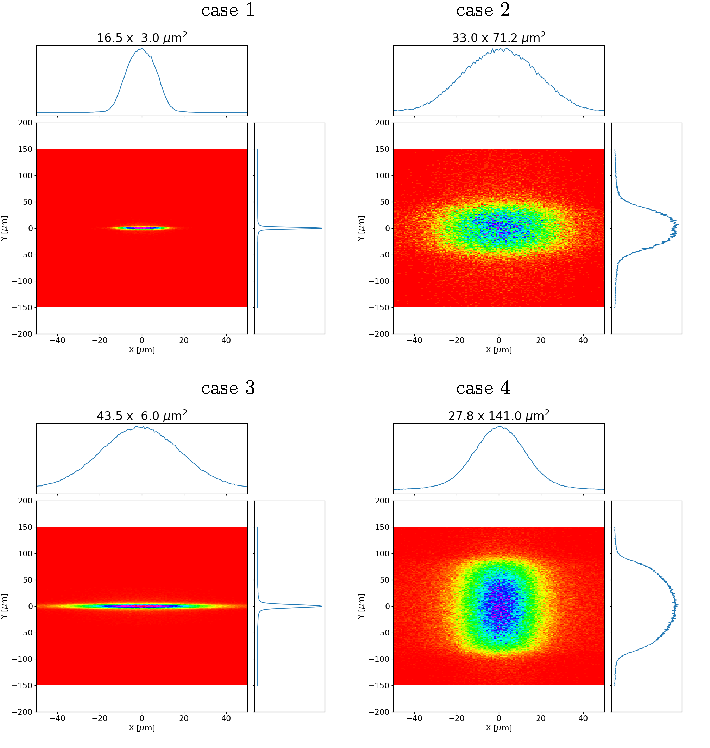
\includegraphics[width=0.99\textwidth]{figures/fig_hybrid.pdf}
    \caption{Hybrid ray-tracing calculations of the intensity distribution at the focal plane for the cases listed in Table~\ref{table:2Dusercases}.}
\end{figure}

\begin{figure}\label{fig:srw}
    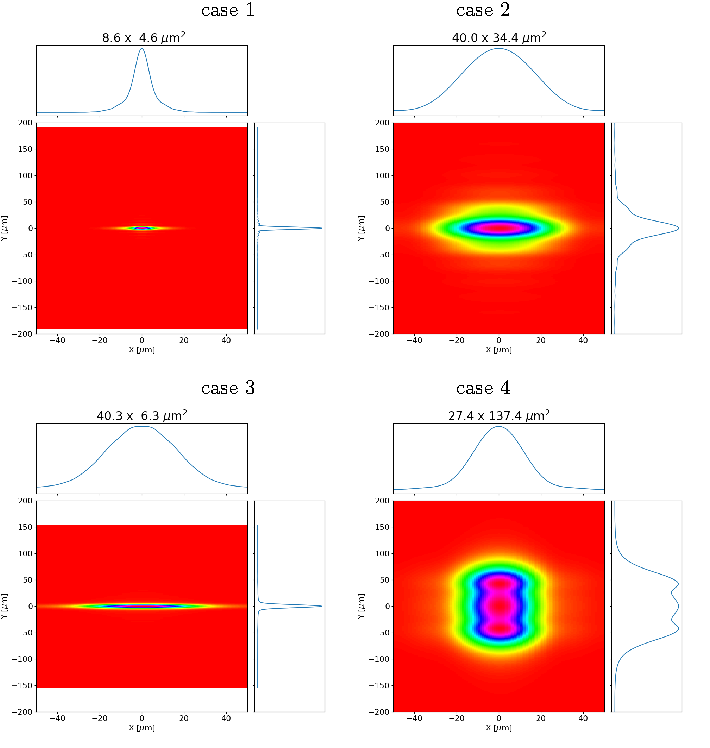
\includegraphics[width=0.99\textwidth]{figures/fig_srw.pdf}
    \caption{Multi-electron SRW calculations of the intensity distribution at the focal plane for the cases listed in Table~\ref{table:2Dusercases}.}
\end{figure}


\begin{figure}\label{fig:comsyl}
    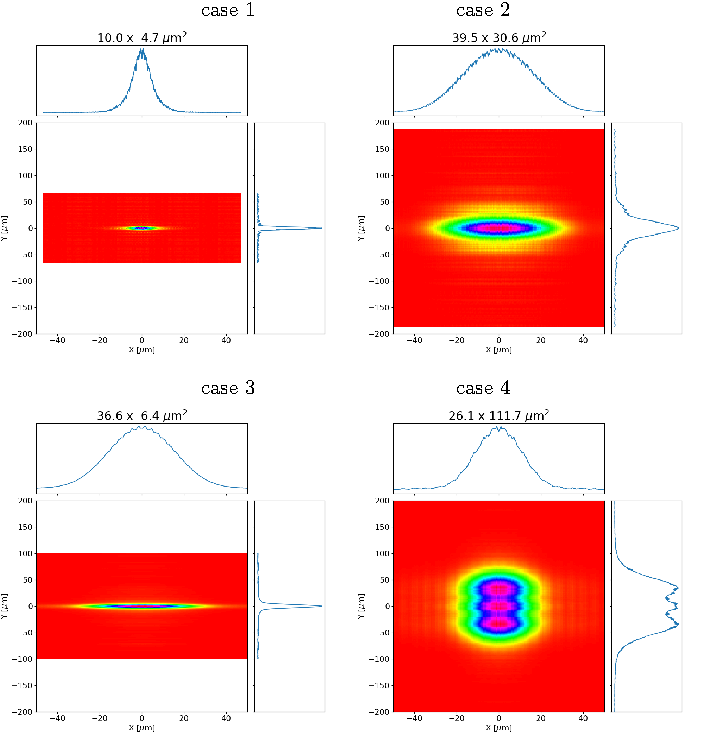
\includegraphics[width=0.99\textwidth]{figures/fig_comsyl.pdf}
    \caption{COMSYL calculations of the intensity distribution at the focal plane for the cases listed in Table~\ref{table:2Dusercases}.
    }
\end{figure}


\begin{figure}\label{fig:2DWofry1D}
    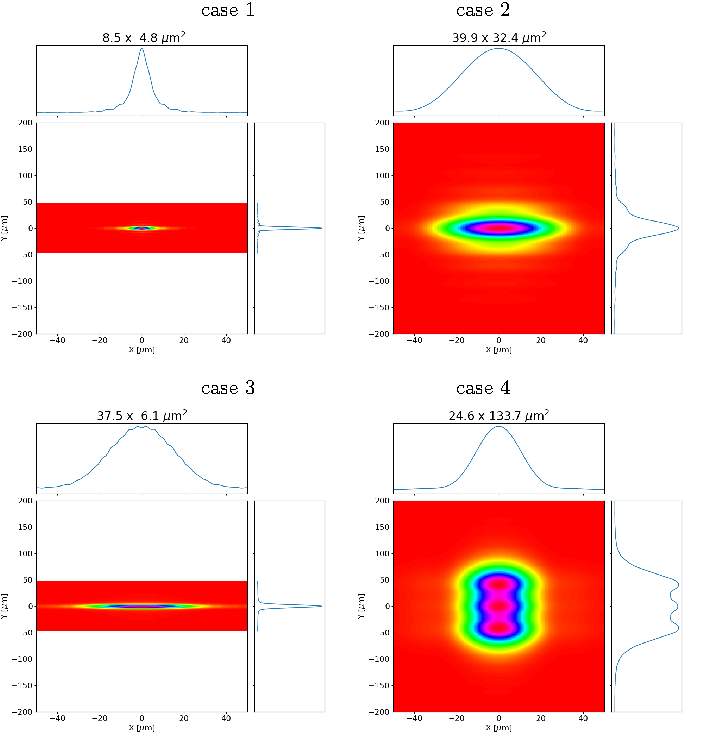
\includegraphics[width=0.99\textwidth]{figures/fig_wofry.pdf}
    \caption{2D intensity distribution at the focal plane. It has been constructed from the Wofry1D calculations.
    }
\end{figure}


\vspace{1cm}




\newpage



\begin{table}[]
    \label{table:comparison}
    \caption{Comparison of sizes (FWHM, in \SI{}{\micro\meter}) calculated with different methods for the cases defined in Table~\ref{table:2Dusercases}.
    In brackets, the values for the fully coherent beam (single electron with SRW, first coherent mode with COMSYL/WOFRY), and zero emittance with Hybrid). \todo{flip columns}
    }
    \centering
    \begin{tabular}{p{0.05\textwidth}|c|c|c|c|c}
         case h/v &
         Wofry1D&
         COMSYL&
         SRW&
         Hybrid \\
         \hline
1 h  & 8.5(8.1)    & 10.0 (9.9)  & 8.6 (7.5)   & 17.3 (17.5) \\
1 v  & 4.8(4.8)    & 4.7 (5.1)   & 4.6 (4.6)   & 3.3 (3.1) \\
\hline
2 h  & 39.9(38.2)  & 39.5 (39.5) & 40.0 (36.1)  & 39.9 (37.5) \\
2 v  & 32.4(29.6)  & 30.6 (29.3) & 34.4 (29.6)  & 74.0 (75.3) \\
\hline
3 h  & 37.5(29.0)  & 36.6 (28.1) & 40.3 (28.4)  & 43.3 (33.0) \\
3 v  & 6.1 (4.9)   & 6.4 (5.7)   & 6.3 (4.6)    & 6.5 (5.8) \\
\hline
4 h  & 24.6(19.1)  & 26.1 (18.6)  & 27.4 (18.0)   & 27.1 (18.8) \\
4 v  & 133.7(110.3)& 111.7 (90.4) & 137.4 (132.0) & 150.2 (159.8) \\
    \end{tabular}
\end{table}

Hybrid ray-tracing for the four cases defined in Table~\ref{table:2Dusercases} are shown in  Fig.~\ref{fig:hybrid}. One can observe that the intensity distributions as not as structured as for the wave-optics methods (e.g. the three-lobe plateau in case 4v is not reproduced). Values of FWHM are in consonance with full wave-optics calculations for most cases (with the exception of two particular cases:
1h (hybrid \SI{16.5}{\micro\meter} Wofry1D \SI{8.5}{\micro\meter}),
2v (\SI{71.2}{\micro\meter} Wofry1D \SI{32.4}{\micro\meter}). They will be discussed in the next section.


SRW-ME results for the four cases are shown in Fig.~\ref{fig:srw}. The good convergence of the values displayed is guarantee by a convergence analysis described in Appendix~\ref{appendix:srw}.
It was used to determine the minimum number of electrons that produce accurate results. The SRW-ME simulations for the cases analyzed converge with only a few thousands electrons, that can be run in less than one hour in a node with 28 CPUs totalizing 256 GB. The reason is that the beam after the slit has a relatively high CF. 


COMSYL requires high performance computing (HPC) to perform full CMD of undulator beam, by
solving the Friedholm problem and obtain the full 2D eigenfunctions (coherent modes) and eigenvalues.
Simulation of the source with COMSYL took 55 min using 28 x 3.30 GHz CPUs of 251.82 GB RAM, for getting 174 modes of 1691 $\times$ 563 pixels.
The modes calculated by COMSYL are loaded in the OASYS environment \cite{codeOASYS} to propagate the modes along the beamline.
The propagation uses 2D zoom propagator and the optical elements available in WOFRY. Results are shown in Fig.~\ref{fig:comsyl}. 
The beam profiles calculated with COMSYL are a bit noisy, which could be improved by increasing the source sampling and further optimizing the propagation parameters. 


WOFRY 1D results are shown in Fig.~\ref{fig:2DWofry1D}. The 1D intensity profile for one direction is obtained from the summation of several modes. High modes have very low eigenvalue and it is enough to consider only 10 modes for reproducing more that 99\% of the spectral density. The 2D intensity distribution shown in Fig.~\ref{fig:2DWofry1D} is obtained combinin the calculated horizontal and vertical 1D profiles via the outer product. We can observe in the intensity distributions the same structures due to the diffraction effects than were observed with the other calculation methods. 
The agreement between the results of  Wofry1D (Fig.~\ref{fig:2DWofry1D}) with SRW (Fig.~\ref{fig:srw}) is striking. All intensity distributions reproduce exactly the same features, and the FWHM values are different in less than 12\%, a value that is compatible with the errors of the simulations (discussed in section~\ref{sec:discussion}). This results validates the 1D CMD method proposed here, whose requirements in computer power are extremely low (it runs very fast in an averaged laptop).  

The specific numeric value for sizes calculated with the different methods (Table~\ref{table:comparison}) depends not only on the code itself, but also on the particular specific parameters in each method (number of pixels for sampling wavefronts, propagation parameters, etc.). To estimate the calculation error in the final size numbers, we vary randomly these specific parameters in a reasonable range (e.g., 10\%). The evaluation of the mean size and the dispersion (standard deviation) of the sizes obtained give an good estimation of the error in this parameter. This exercise would take a considerable computational effort using 2D methods, but it can be easily done with Wofry1D. We run 200 cases with 10\% random variation in the values in number of pixels and magnification factor in drift spaces. The obtained sizes (horizontal $\times$ vertical) are  
8.49 $\pm$ 0.60 $\times$ 4.97 $\pm$ 0.37 \SI{}{\micro\meter}$^2$ (case 1),
39.94 $\pm$ 2.98 $\times$ 32.77 $\pm$ 2.69 \SI{}{\micro\meter}$^2$ (case 2),
36.39 $\pm$ 2.89 $\times$ 6.12 $\pm$ 0.51 \SI{}{\micro\meter}$^2$ (case 3), and
24.18 $\pm$ 1.80 $\times$ 133.44 $\pm$ 10.06 \SI{}{\micro\meter}$^2$ (case 4). We confirmed that the values given in Fig.~\ref{fig:2DWofry1D} are within these error intervals.


The calculated beam sizes should be completed with flux. At \SI{7}{keV}, the undulator in the configuration selected emits a flux of 1.5 10$^{15}$ photons/s/0.1\%bw. Each of the three elements studied (slit, lens -1 and lens-2) absorb part of the flux. The estimation of the absorption by the slit can be done using simple geometrical arguments, and the absorption by the slits depend on the average Be thickness presented to the beam. The linear attenuation coefficient of Be at 7 keV is $\mu=$~\SI{3}{\centi\meter}$^{-1}$, giving 1.45\% attenuation for a \SI{50}{\micro\meter} thick layer (like lens thickness used in simulations\footnote{In the simulations the horizontal and vertical focusing are separated in two lenses, with accumulated thickness \SI{100}{\micro\meter} thus absorption 3\%}). For the case 1 simulations we extracted the absorption for the different absorbing elements (slit, lens-1 and lens-2) in the case of partial coherence and also for full coherence (see Table~\ref{table:absorption}).
There is excellent agreement for partial coherence. For full coherence, the Wofry1D results are different than the SRW+Hybrid, because the geometry of the 1st coherent mode used to represent the full coherent beam is not the same as the geometry of the filament beam (used in SRW and Hybrid). We note a high absorption in lens-2, due to the fact that in this case the lens-2 is overilluminated, therefore the \SI{1}{\milli\meter} physical aperture absorbs considerably the beam.

\begin{table}[]
    \label{table:absorption}
    \caption{Comparison of beam intensity attenuation in percent by the slit, lens-1 and lens-2 for the partial coherent beam, 
    % coherent beam (first coherent mode in Wofry1D, filament beam in SRW, zero emittance in Hybrid) and for the partial coherent beam,
    for the four cases studied.
    The Wofry1D data shown here comes after combining the horizontal and vertical wavefronts using the outer product. 
    }
    \centering
\begin{tabular}{l|lll|lll|lll}
case & \multicolumn{3}{c|}{slit} & \multicolumn{3}{c|}{lens-1} & \multicolumn{3}{c|}{lens-2} \\
\hline
     & \rot{Wofry1D} & \rot{SRW} & \rot{Hybrid}
     & \rot{Wofry1D} & \rot{SRW} & \rot{Hybrid}
     & \rot{Wofry1D} & \rot{SRW} & \rot{Hybrid}
\\
\hline
%    &          &      &        &          &      &         &          &       &         \\
%1      &   87.0   & 96.6 & 96.7   & 7.6      & 7.4  & 5.2     & 48.3     & 51.3  & 53.0   \\
1       &   97.6   & 97.6 & 97.2   & 7.9      & 7.6  & 5.2     & 50.7     & 51.1  & 52.6   \\
% 2c    &   87.0   & 96.6 & 96.7   & 6.7      & 6.4  & 4.3     & 3.8      & 3.7   & 3.3    \\
2       &   97.6   & 97.6 & 97.2   & 7.0      & 6.6  & 4.3     & 3.9      & 3.7   & 3.3    \\
% 3c    &   55.9   & 86.0 & 85.6   & 5.4      & 6.11 & 4.7     & 17.1     & 22.7  & 26.6   \\
3       &   89.5   & 90.2 & 88.6   & 6.3      & 6.1  & 4.6     & 23.4     & 21.8  & 25.2   \\
% 4c    &   55.9   & 86.0 & 85.6   & 6.8      & 7.73 & 6.4     & 3.6      & 3.6   & 3.6    \\
4       &   89.5   & 90.2 & 88.6   & 8.0      & 7.7  & 6.2     & 3.8      & 3.6  & 3.6   \\
\end{tabular}
\end{table}


\section{Discussion}
\label{sec:discussion}

% Our discussion follows a hierarchical approach, as discussed in \citeasnoun{hierarchical}, with the idea of balancing accuracy and computational effort, to subsequently select and use the most advantageous method for the analyzed problem. 
% This multi-method analysis will also help to validate the new 1D CMD method introduced in this work. The results of the Wofry1D results are compared with other well-known simulation packages. 


There is good agreement in focal size FWHM values in all methods (see Table~\ref{table:comparison}), but also in the shape of intensity distributions, in particular for the wave optics methods (compare Figs. ~\ref{fig:2DWofry1D}, ~\ref{fig:comsyl} and ~\ref{fig:srw}). 

Regarding computer resources, the Wofry1D code can be run in a few seconds in a laptop, whereas the simulation of the full CMD with COMSYL required about 1h (for 1691 x 563 pixels, 174 modes) using 1 node of 28 cores. This source is then reused for propagating the different configurations. Each configuration required a full SRW-ME with 5000 electrons run in also about 1h in a similar configuration. 

% \subsection{Hybrid ray-tracing}

% The simulation results for the four cases studied using the hybrid method indicate that, although this method does not reproduce exactly the intensity distibution given by full partial coherent optics, the numerical values are approaching the good ones, but with two exceptions: the case 
% 1h (hybrid \SI{16.5}{\micro\meter} Wofry1D \SI{8.5}{\micro\meter}) and the case 
% 2v (\SI{71.2}{\micro\meter} Wofry1D \SI{32.4}{\micro\meter}). 
% We remark that these thee cases have in common that the $f_1$ value in use is close to $f_1$~=~\SI{40}{\meter} that corresponds to the singularity in the analytical (geometrical optics) calculations, when the lens-1 focuses on lens-2. A detailed study with hybrid was performed to calculate the FWHM for all possible values of $f_1$ (as done in Fig.~\ref{fig:focalSizes}. The result (Fig.~\ref{fig:focalSizes_hybrid}) confirms that there is good agreement everywhere except in the region close to $f_1$~=~\SI{40}{\micro\meter}.
% We thus conclude that the hybrid ray-tracing is a valid method to obtain good values of focal sizes in most cases, excepts for the case that lens-1 focus is close to the position of lens-2 ($f_1 \approx $~\SI{40}{\meter}).


% \begin{figure}
%     \centering

%     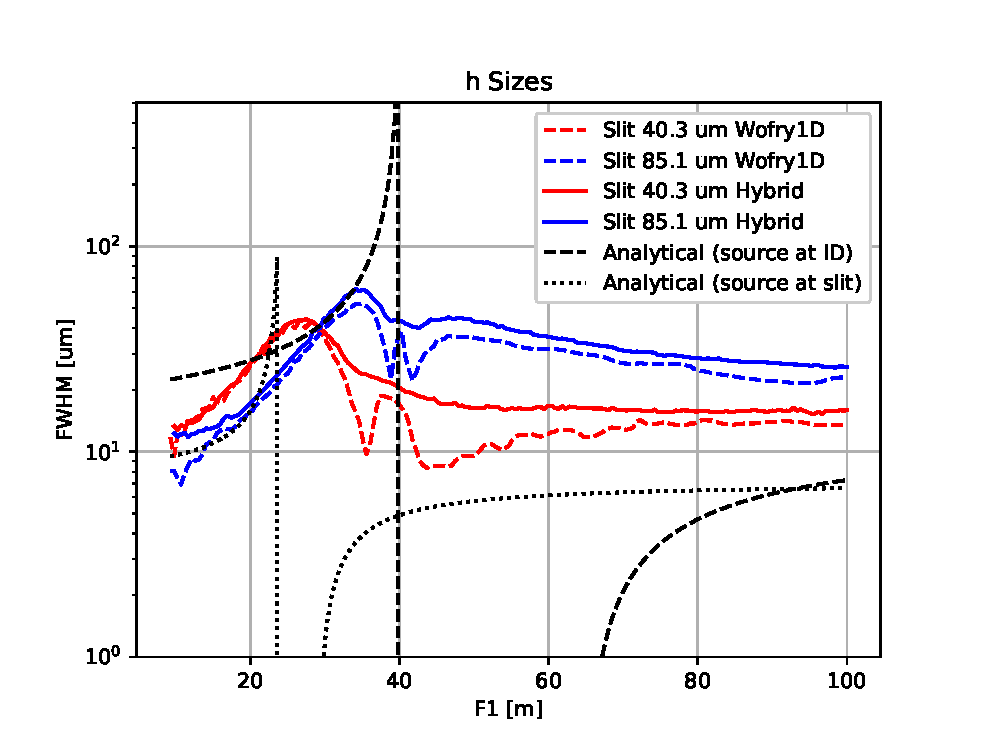
\includegraphics[width=0.95\textwidth]{figures/sizes_h_hybrid.eps}
%     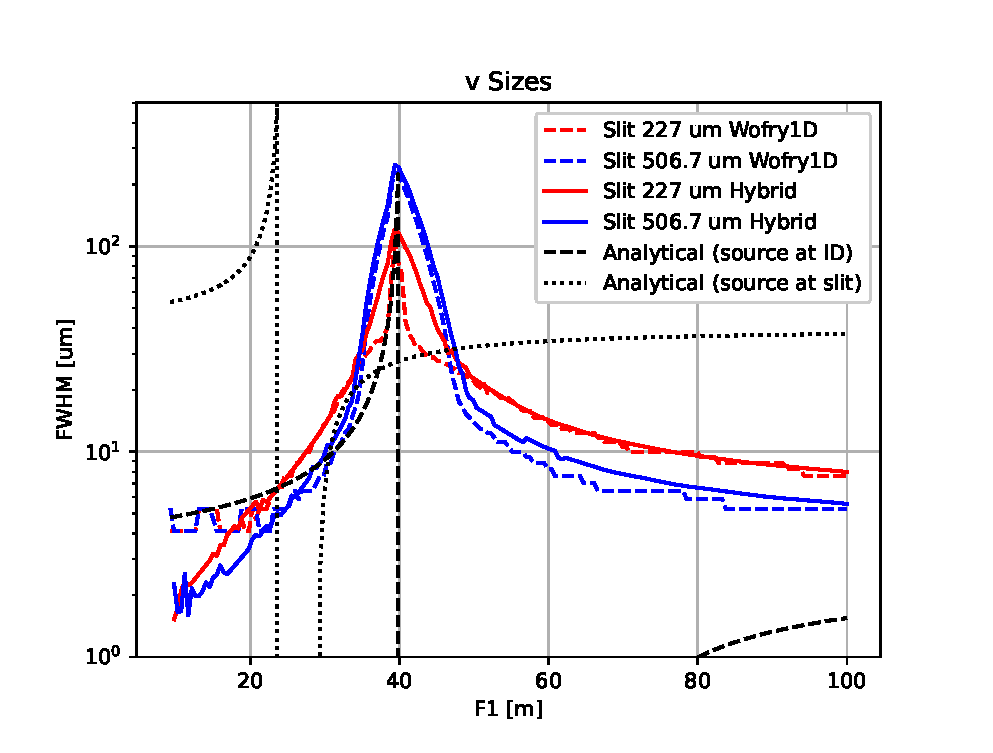
\includegraphics[width=0.95\textwidth]{figures/sizes_v_hybrid.eps}
        
%     \caption{Focal sizes obtained by hybrid ray-tracing method, for two slit aperture cases, compared with values from Wofry1D  (from Fig.~\ref{fig:focalSizes}).}
%     \label{fig:focalSizes_hybrid}
% \end{figure}

% \subsection{Further simulations}

The simulations presented, motivated by the ID18 project, use a simplified optical layout. A more complete study including the other optical elements, other transfocator configurations will be presented elsewhere, also for different energies and implementing the effect of surface errors due to thermal load and surface finish. 

We have also calculated the beam evolution in the neighbourhood of the sample position for the four cases studied (see Fig.~\ref{fig:caustic}). From these plots one can obtain the position of the best focus and the depth of focus. The depth of focus (measured as the distance where the peak value is reduced by 15\%) is larger than two meters (except for the cases 1v, 3v). \todo{redo these plots and compare with SRW... otherwise supress?}

% In some cases there is a mismatch between the position of the best focus and its expected position (the sample position, at the zero abscissas). This effect, certainly due to an error in setting $f_2$, may have several origins. 

% For pairing two transfocators, the algorithm chosen to calculate the $f_2$ value consist in analyzing the wavefront at the lens-2 position, find a corrector refractive object that would transform the incoming wavefront in a converging wavefront (see section \ref{sec:refractorCorrector}), and fit the radius at the center. We then get the $R_2$ and therefore the $f_2$ value. In addition, to obtain smooth $(f_1,f_2)$ curves in Fig.~\ref{fig:f1f2map} we have used a Gaussian slit (see section \ref{sec:gaussianslit}). It smears out the diffraction fringes, because in an ideallized system where a point source is focused at the sample position, the recorded intensity would correspond to the diffraction pattern of the slit, that can be considered as an "object" placed in the beam (see e.g. \cite{paganin_book}). The use of a Gaussian object implies that its diffraction pattern is a Gaussian with no diffraction fringes. 

% For cases 1h, 1v, 3v (see  Fig.~\ref{fig:caustic}), there is a good agreement between the focal position obtained from the maximum of intensity on-axis (plotted at the top of the image) and our expected position (the zero in the plots). In some other cases (2v, 3h, 4h) the agreement is acceptable, taking into account that the observed depth of focus is of the order of meters. A small correction in $f_2$ would bring the best focus to its ideal position. This correction is necessary because we used a Gaussian slit for calculating $f_2$, thus neglecting some oscillations around the $(f_1,f_2)$ curves. There are two pathological cases where the algorithm used to calculate $f_2$ did not succeed: the cases 2h and 4v.
% The error in $f_2$  for case 2h is also due to the oscillations in the $(f_1,f_2)$ and can be corrected, as shown in Fig.~\ref{fig:causticcorrection}a. However, case 4v cannot be corrected because we would need a divergent lens to bring the focus of $f_1$ to the sample position. Setting $R_2=f_2=\infty$ would reduce the beam size at the sample position (Fig.~\ref{fig:causticcorrection}b), but cannot get the best focus there. However, an ad-hoc defined refractive corrector in the place of lens-2 would do the job (Fig.~\ref{fig:causticcorrection}d).  

 



%%%%%%%%%%%%%%%%%%%%%%%%%%%%%%%%%%%%%%%%%%%

\begin{figure}\label{fig:caustic}
\centering

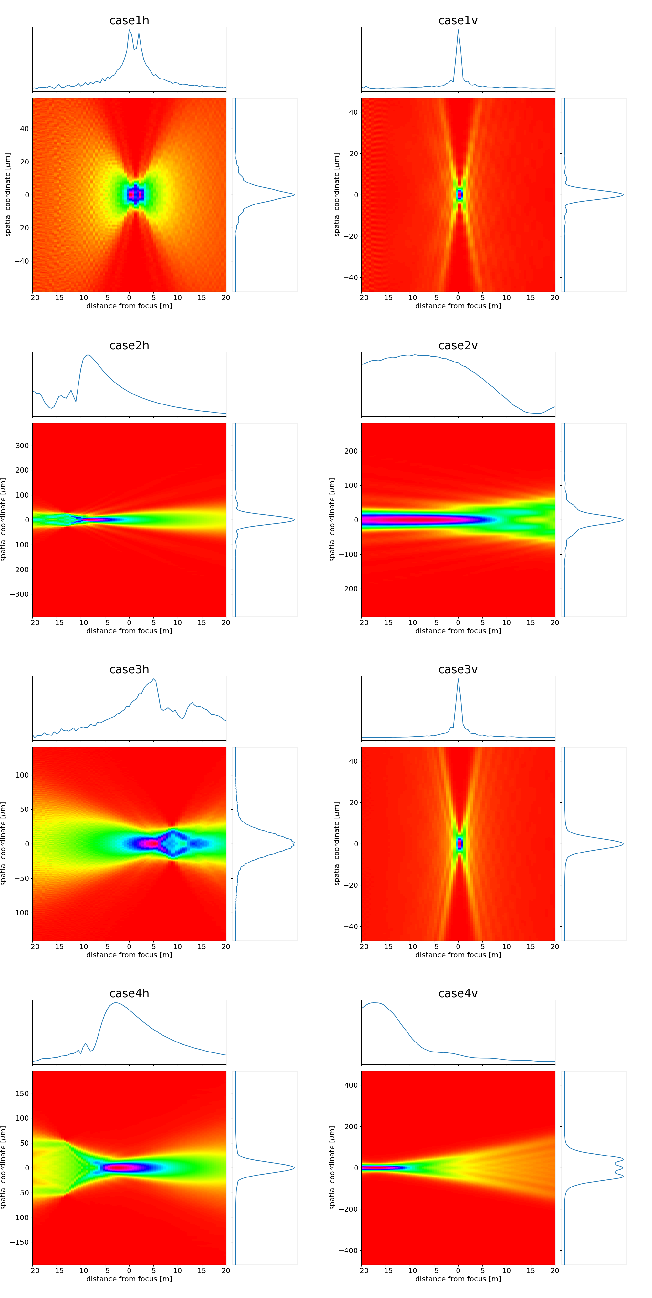
\includegraphics[width=0.99\textwidth]{figures/fig_caustic.pdf}

\caption{Evolution of the beam size in the around the sample position for the cases listed in Table~\ref{table:2Dusercases}. The top and side graphs correspond to the profiles passing by (0,0).
}
\end{figure}



% \begin{figure}\label{fig:causticcorrection}
% \centering
% 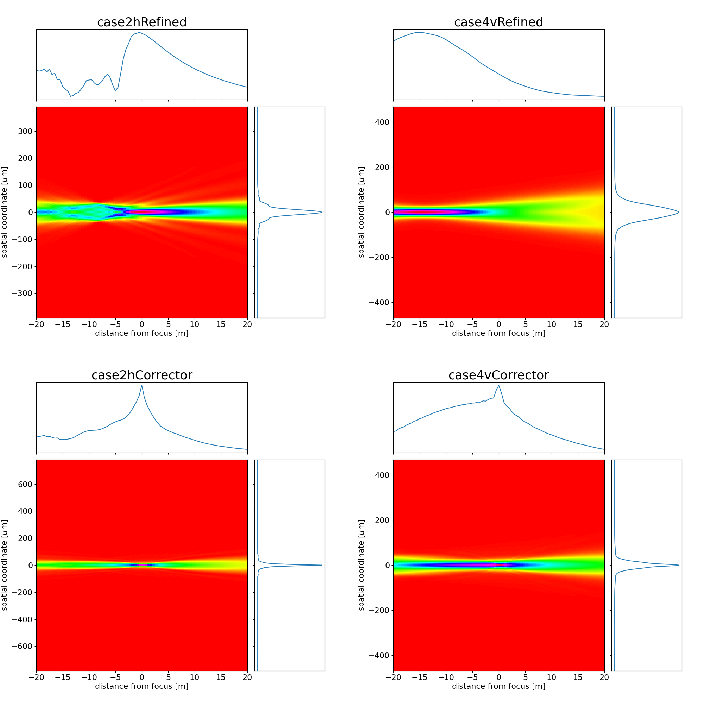
\includegraphics[width=0.99\textwidth]{figures/fig_caustic_correction.pdf}

% \caption{Evolution of the beam size in the around the sample position for the ``pathological" case 2h and 4v shown in Fig.~\ref{fig:caustic}. Top row: using corrected lens-2 with $R_2$=\SI{410}{\micro\meter} ($f_2=$\SI{29.4}{\meter}) for case 2h and $R_2=f_2=\infty$ for case 4v. Bottom: using a free-form refractive corrector instead of lens-2.
% }
% \end{figure}


% \subsection{Errors in optical surfaces}

% % \todo{Rafael, please re-read}
% The performance of X-ray optics in the new generation synchrotron beamlines is limited by the quality of the optical surfaces \cite{lengeler1999,Yabashi}. Finish errors can be divided in three families: i) height errors, associated with surface finishing (high spatial frequency), ii) figure errors, associated with deviations from ideal profile (e.g. bending, gravity sag, thermal deformations), and iii) slope errors or waviness, associated to medium spatial frequencies \cite{srio1992, signorato1997}. Finish errors in x-ray lenses can be measured by different techniques (eg. grating interferometry, x-ray speckle tracking or ptychography) and readily included in the simulations \cite{Celestre:mo5214}. Some profiles measured at ESRF using x-ray speckle tracking \cite{berujon2020} with height error RMS of the order of \SI{1}{\micro\meter} are used to verify that the focal spot produced by lenses with realistic errors is not degraded with respect to the ideal lens surface. 

% Usually the optics of new generation synchrotron beamlines is limited by the quality of the optical surface. Typically are due to surface finish (slope errors and height errors) and shape errors, often due to heat load. 
% \todo{Rafael, would you please work next paragraph. I checked that your error file (profile 1 in DABAM2D) does not produce relevant changes, thus the idea is to "mention" the errors without presenting a full study.} Surface errors in lens surfaces can be experimentally measured by different techniques (e.g. speckle tracking, ptychography) and included in the simulations. Some profiles measured at ESRF \cite{???} with height error RMS of the order of \SI{1}{\micro\meter}  are used to verify that the focal spot produced by lenses with realistic errors is not degraded with respect to the ideal lens surface. 

% The effect of finish errors in the white double-mirror system is also analyzed using a measured mirror meridional profile of \SI{2.5}{\nano\meter} height error RMS and \SI{140}{\nano\radian} RMS slope error. 

% % \todo{Philipp, please re-read}
% The heat load affect several elements of the beamline. For the beamline under consideration, the affected elements (white beam mirrors, and double-crystal monochromators) are not presented in our simulations. Finite element analysis of mirrors and crystals done for other EBS beamlines \cite{Brumund} show that the deformation height profile can be decomposed it two parts: an average bending that is possible to correct by a small readjustment of the focal length of the optical elements downstream the heated element, and a ``residual error" which remain after removing the averaged bending radius, and could only be corrected using adaptive optics. Wofry1D simulations using FEA-generated deformations at the first crystal of a monochromator placed just after the coherent slit showed no significant degradation of the focal spot, both in size and shape. This is mainly due to the low power transmitted by the coherent slit. We checked that the focused beam is almost unchanged when using a profile from FEA analysis with curvature of about \SI{1}{\kilo\meter} and residual slope errors of \SI{30}{\nano\radian}. 



% The deformation profile calculated by FEA \todo{I USED FILE: SRC\_Si\_3.0mrad\_08000eV\_mo\_Si111\_Size1\_nodalOut.out} is is loaded in a ``mirror-like" element in Wofry, as described \cite{srioLBL}. For case 1, a small degradation in the horizontal direction is found (passing from \SI{8.09}{\micro\meter} to \SI{10.21}{\micro\meter} for the first coherent mode). It is accompanied by a loss of symmetry. A large deformation in the vertical spot is observed, but a spot close to the ideal is found when a best circle is subtracted from the profile. It is then possible to correct this added curvature. Indeed, by adjusting $f_2$ \todo{I will calculate this} it is possible to compensate the effects introduced by the crystal bending due to heat load.


% finding focus https://www.optikos.com/finding-focus/

% \subsection{Practical considerations} Simulations like those presented here could be very beneficial for beamline operation, for its optimization and quick setting.  Complicated  relationships exist between the beam parameters requested by users (beam size and coherent fraction) and the beamline configuration (undulator, slit and transfocator setting). Quick simulations as done by Wofry1D could be a helpful instrument for the beamline staff to get the desired configurations. The plots shown here (e.g., $CF$ vs slit size in Fig.~\ref{fig:cf_vs_aperture}, trajectories in Fig.~\ref{fig:f1f2map}, or final size in Fig.~\ref{fig:focalSizes} could be simulated on-line and compared with results presented as look-up tables with similar aspect. We are also considering the design of a digital twin that mimics the real transfocator systems to assist beamline setting. For that, the fast simulation using the CMD method developed in Wofry1D will be an integrated component.  

% Some practical consequences can be directly deduced from the results shown here. For example, looking at Fig.~\ref{fig:focalSizes} one can observe that the same focal size can be obtained with different configurations. To get a similar size, it is better to prefer a large $f_1$ to avoid over-illuminating the lens-2 and increase transmission of lens-1. The transfocator design is simplified if we restrict the horizontal focal distance t to be smaller than the vertical $f_h>f_v$. Here, $f_v$ can be obtained with lenses focusing in 2D and $f_h$ by adding 1D lenses focusing in the horizontal plane. 

% % https://www.optikos.com/finding-focus/
% In this work we configured the transfocator to have the resulting focal position on the sample plane, an "in-focus" setup. It could also be possible to work off-focus to vary the beam size at the sample plane. The in-focus setup will generally produce the sharpest image of very small details in the image. Moreover, it will reduce the artifacts produced by the surface finish errors. Also, a larger depth of focus is obtained at this position (see e.g. Fig.~\ref{fig:causticcorrection}).


\section{Summary and conclusions}
\label{sec:summary}

We have studied a particular case of focusing a partial coherent beam (as produced by the low emittance storage ring EBS-ESRF) by a system of two transfocators (or lenses). We have verified that four simulation codes typically used to simulate synchrotron beamlines agree in the results of beam size and flux. The hybrid ray-tracing method (ShadowOUI) fails to determine fine structures in the beam intensity profiles. The three codes using physical optics (SRW-ME, COMSYL and WOFRY1D) produce essentiually the same results. Partial coherence calculations using 2D wavefronts are expensive from the computation point of view, either because many thousands of wavefronts are propagated (in SRW-ME) or because the need of diagonalizing an extremely large 4D cross spectral function. The newly developed coherent mode decomposition of 2D CSFs (i.e. separating 1D modes for the horizontal and vertical direction) is very rapid and can be run interactively in a laptop. Its results for the particular cases simulated here agree very well with full 2D propagation methods. 
This method is available in the Wofry add-on of the OASYS suite \cite{codeOASYS}. OASYS workspaces for the simulations performed in this paper are available\footnote{{ https://github.com/oasys-esrf-kit/paper-multioptics-resources}}.

% Four cases are calculated and compared using the other methods available in OASYS, like the full 2D coherent mode decomposition using COMSYL \cite{codeCOMSYL}, the OASYS interface for the SRW \cite{codeSRW} code, and hybrid ray-tracing \cite{codeHYBRID}.


%%%%%%%%%%%%%%%%%%%%%%%%%%%%%%%%%%%%%%%%%%%%%%%%
%%%%%%%%%%%%%%%%%%%%%%%%%%%%%%%%%%%%%%%%%%%%%%%%
%%%%%%%%%%%%%%%%%%%%%%%%%%%%%%%%%%%%%%%%%%%%%%%%
\appendix


\section{Some considerations on partially-coherent calculations using SRW's macro-electrons \& simulation convergence}
\label{appendix:srw}



The convergence of the SRW-ME method is based on the \textit{finesse} with which the distribution $f(\textbf{s}_\text{e}, \textbf{s}'_\text{e}, \gamma_\text{e})$  in equation~(\ref{eq:SR}) is sampled. While an exquisitely large number of \textit{me's} will lead to a more accurate simulation, the resulting calculation would be very long and impossible to be performed on personal computers within reasonable time even if performed in parallel. The number of \textit{me's} depends on overall beamline degree of coherence at the observation plane, which is impacted by the source coherent fraction and beamline overall transmission (eg. slits, creation of secondary sources or any other spatial filtering scheme). Special attention to the number of macro-electrons should be given if the simulation accounts for vibrations in the beamline elements or broad-band radiation (eg. pink beam or radiation filtered by multi-layer monochromators).

To illustrate the effect of the number of macro-electrons on the beam profile we choose the previously studied cases 1 and 3 from section~\ref{sec:complete-beamline} - due to their $CF$, cases 2 and 4 are expected to have the same convergence as 1 and 3, respectively. Both systems 1 \& 3 (and 2 \& 4) have the same X-ray source and are illuminated up until the slits (36~m downstream U18) by the same beam, differing mainly by the coherent fraction selected for the rest of the beamline with case 1 having a higher $CF$ than case 3 - refer to Tables~\ref{table:id18parameters} and \ref{table:2Dusercases} for the complete simulation parameters. The results for a selected number of \textit{me's} are shown in Figs.~\ref{fig:me_c1} and \ref{fig:me_c3}. The 1 \textit{me} simulation represents the filament-beam source, where the electron beam emittance is negligible and the fully spatial coherence is assumed - this is often called a ``single electron simulation". On the other extreme, an exaggerated value of 100k $me's$ is chosen as a way of guaranteeing convergence by brutal-force. Two criteria are used to evaluate the convergence of the simulations: the beam shape and peak intensity stabilisation. The profile cuts in  Fig.~\ref{fig:me_c1}(a)-(b) and Fig.~\ref{fig:me_c3}(a)-(b) show that the profile shape starts to converge to that of a 100k $me's$ after $\sim$500 macroelectrons for case 1 and $\sim$1k macroelectrons for case 3. Beyond that, it is necessary to resort to the relative error standard deviation and the peak intensity stabilisation. Fig.~\ref{fig:me_c1}(c)-(d) and Fig.~\ref{fig:me_c3}(c)-(d) show that for both cases, the convergence happens between 2k and 5k $me's$. Further increase in the number of macro electrons does not translate in improvements in the simulations (see simulations for 10k $me's$ onward), but increase greatly the cost of the calculation as shown in Fig.~\ref{fig:me_t}. For the work presented here a good compromise between accuracy and efficiency of the calculations is reached at 5k $me's$. Other factors contributing to the total elapsed simulation time and overall parallel performance of SRW-ME method are presented in \S3.3 from \cite{codeSRW_MEscan}, but these do not impact the SRW-ME convergence.

It is important to note that this large scan procedure is merely illustrative. Usually an experienced optical designer starts with a good guess of the necessary number of $me's$ based on the characteristics of the source (degree of coherence) and optical system (transmission and expected degree of coherence at the observation plane). This choice usually includes considerations of time and resources consumption. If there are signs that the choice may be too low, further attempts with higher $me's$ should be done. If the simulation looks fine from the first guess, reducing the number of $me's$ is also interesting as very often it is necessary to repeat the simulations (eg. testing different configurations, different energies, tolerancing or even different observation planes). At the time of writing, the authors are unaware of any widespread metric within the SRW's community capable of giving the exact number of \textit{me's} necessary for the convergence of the SRW-ME method other than the $me's$ scan. We welcome the discussion on SRW-ME convergence and we encourage the reader to reach out if they employ any interesting and reproducible convergence metric that is less time (and resource) consuming.

% \begin{table}[]
% \label{table:me_t}
% \caption{Time}
% \resizebox{\textwidth}{!}{
% \begin{tabular}{cccccccc}
%  & 500 & 1k & 2k & 5k & 10k & 25k & 100k \\ \hline
% case 1: & 5min & 9min & 15min & 39min & 1h20min & 3h21min & 13h15min \\
% case 3: & 9min & 17min & 30min & 1h15min & 2h35min & 6h30min & 35h39min
% \end{tabular}}
% \end{table}

\begin{figure}
    \centering
    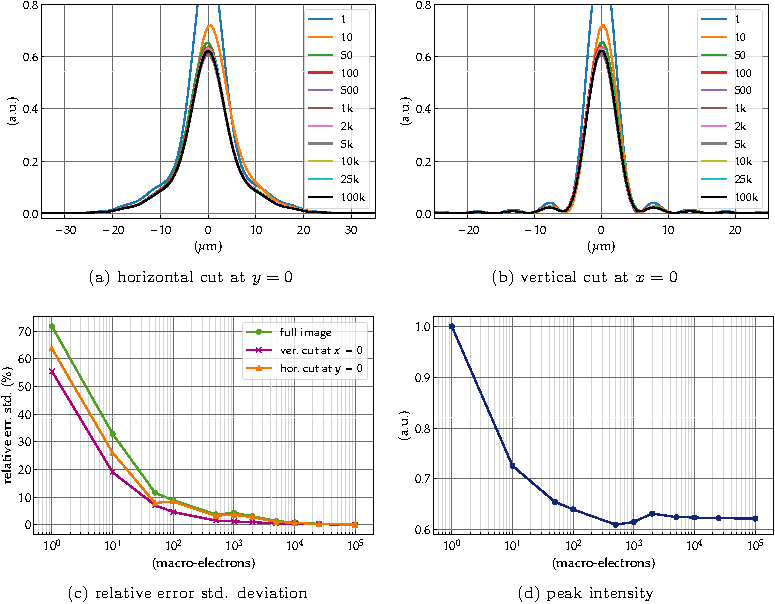
\includegraphics[width=\textwidth]{figures/c1.pdf}
    \caption{Partially-coherent simulations convergence study: case 1. (a) horizontal and (b) vertical intensity cuts at E=7~keV for $me's$ ranging from 1 to 100k. (c) errors relative to the $me's=$100k plots and (d) peak intensity.}
    \label{fig:me_c1}
\end{figure}

\begin{figure}
    \centering
    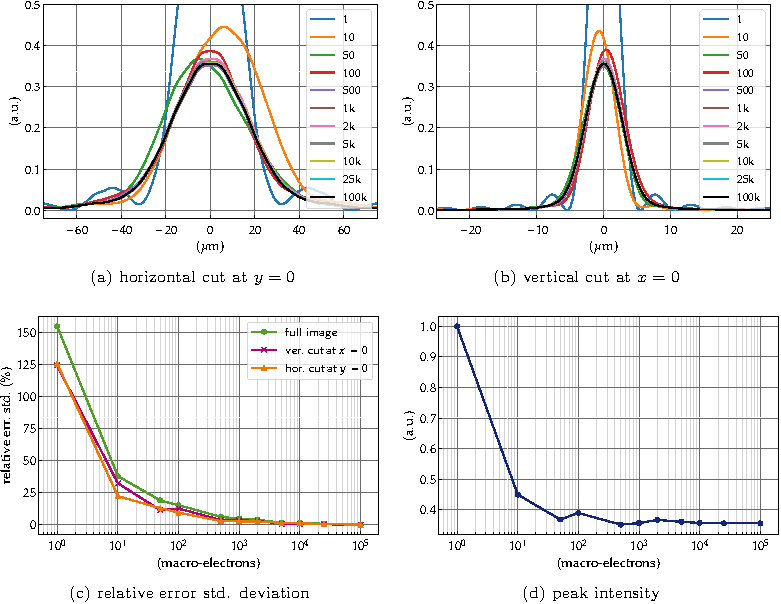
\includegraphics[width=\textwidth]{figures/c3.pdf}
    \caption{Partially-coherent simulations convergence study: case 3. (a) horizontal and (b) vertical intensity cuts at E=7~keV for $me's$ ranging from 1 to 100k. (c) errors relative to the $me's=$100k plots and (d) peak intensity.}
    \label{fig:me_c3}
\end{figure}

\begin{figure}
    \centering
    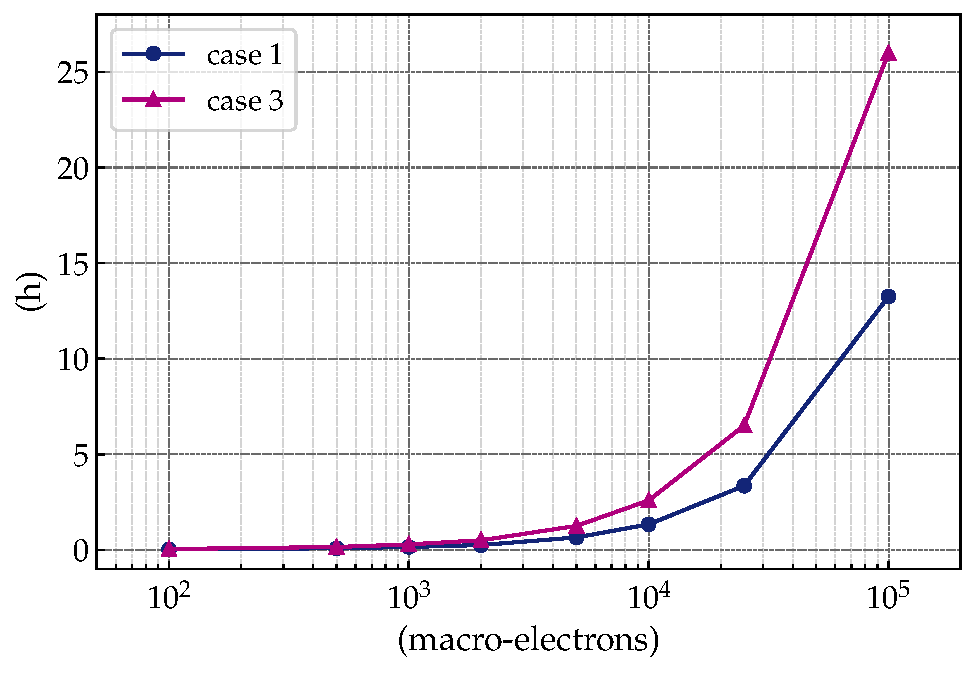
\includegraphics[width=0.8\textwidth]{figures/srw_time.pdf}
    \caption{Total elapsed time for partially-coherent simulations using a computer cluster with 28 processors for parallel calculations as a function of number of $me's$.}
    \label{fig:me_t}
\end{figure}

\newpage
% %%%%%%%%%%%%%%%%%%%%%%%%%%%%%%%%%%%%%%%%%%%%%%%%
% %%%%%%%%%%%%%%%%%%%%%%%%%%%%%%%%%%%%%%%%%%%%%%%%
% %%%%%%%%%%%%%%%%%%%%%%%%%%%%%%%%%%%%%%%%%%%%%%%%

 %-------------------------------------------------------------------------
 % The back matter of the paper - acknowledgements and references
 %-------------------------------------------------------------------------

 % Acknowledgements come after the appendices

\ack{\textbf{Acknowledgements}}

This project has received funding from the European Union’s Horizon 2020 Research and Innovation programme under grant agreements N$^{\circ}$ 823852 (Photon and Neutron Open Science Cloud -- PaNOSC) and N$^{\circ}$ 101007417 (NFFA-Europe Pilot Joint Activities -- NEP).
%. R.C. acknowledges funding from the European Union’s Horizon 2020 research and innovation programme under grant agreement N$^{\circ}$ 101007417 within the framework of the NFFA-Europe Pilot Joint Activities.




\referencelist{iucr}

 %-------------------------------------------------------------------------
 % TABLES AND FIGURES SHOULD BE INSERTED AFTER THE MAIN BODY OF THE TEXT
 %-------------------------------------------------------------------------

     

\end{document}                    % DO NOT DELETE THIS LINE
%%%%%%%%%%%%%%%%%%%%%%%%%%%%%%%%%%%%%%%%%%%%%%%%%%%%%%%%%%%%%%%%%%%%%%%%%%%%%%
